
% this file is called up by thesis.tex
% content in this file will be fed into the main document

%: ----------------------- introduction file header -----------------------
\chapter{Experiments}\label{ch:experiments}

\graphicspath{{experiments/figures/}}

% -------------------------------------------------------------
% -- Experiments
% -------------------------------------------------------------

The hypotheses raised in this thesis have been further validated in real projects. The implementation of the proposed algorithms and their execution in systems used by third parties, has allowed us to verify the results obtained during the evaluations. Some of these projects are framed in the health field, specifically in the area of HIV treatment (Section \ref{sec:polypharmacy}) and, recently, in the field of COVID-19 treatment (Section \ref{sec:drugs4covid}). In both cases our algorithms have helped to analyze the use of drugs to treat diseases. There are also projects aimed at measuring the impact of scientific research, at a national level through the creation of patents and research collaborations (Section \ref{sec:corpus-viewer}), and by research area from a point of view of originality and creativity of research (Section \ref{sec:drinventor}). Finally, the results of this thesis have also been used to facilitate the exploration of public procurement data in Europe (Section \ref{sec:tbfy}). Tenders performed by public administrations across Europe were related in an automatic and language-independent way to facilitate their exploration and allow local administrations to know how similar processes are managed in other countries.  


\section{Polypharmacy and Drug-drug Interactions}
\label{sec:polypharmacy}

Does the number of concomitant drugs in people living with Human Immunodeficiency Virus (HIV) increase with age and is it greater than in non-HIV-infected persons? This research question \citep{Badenes-Olmedo2019c} seems to be far from the scope of this thesis. However, if we take into account that  concomitant drugs are the drugs that a patient also uses to treat other diseases, we can draw an analogy to bring it closer to our domain. It aims to analyze patients from the medicines they receive, and our algorithm organizes documents described by topics. A patient, seen as a document, is described by the drugs he/she receives to treat HIV, which can be represented as topics, and the drugs he/she receives to treat other diseases (i.e concomitant drugs) , which would be used to set the relevance of each topic from their interactions. The relationships between patients depend on the drugs they share, and can be measured by the topics they share when they are represented as documents.


\begin{figure}[ht]
    \centering
    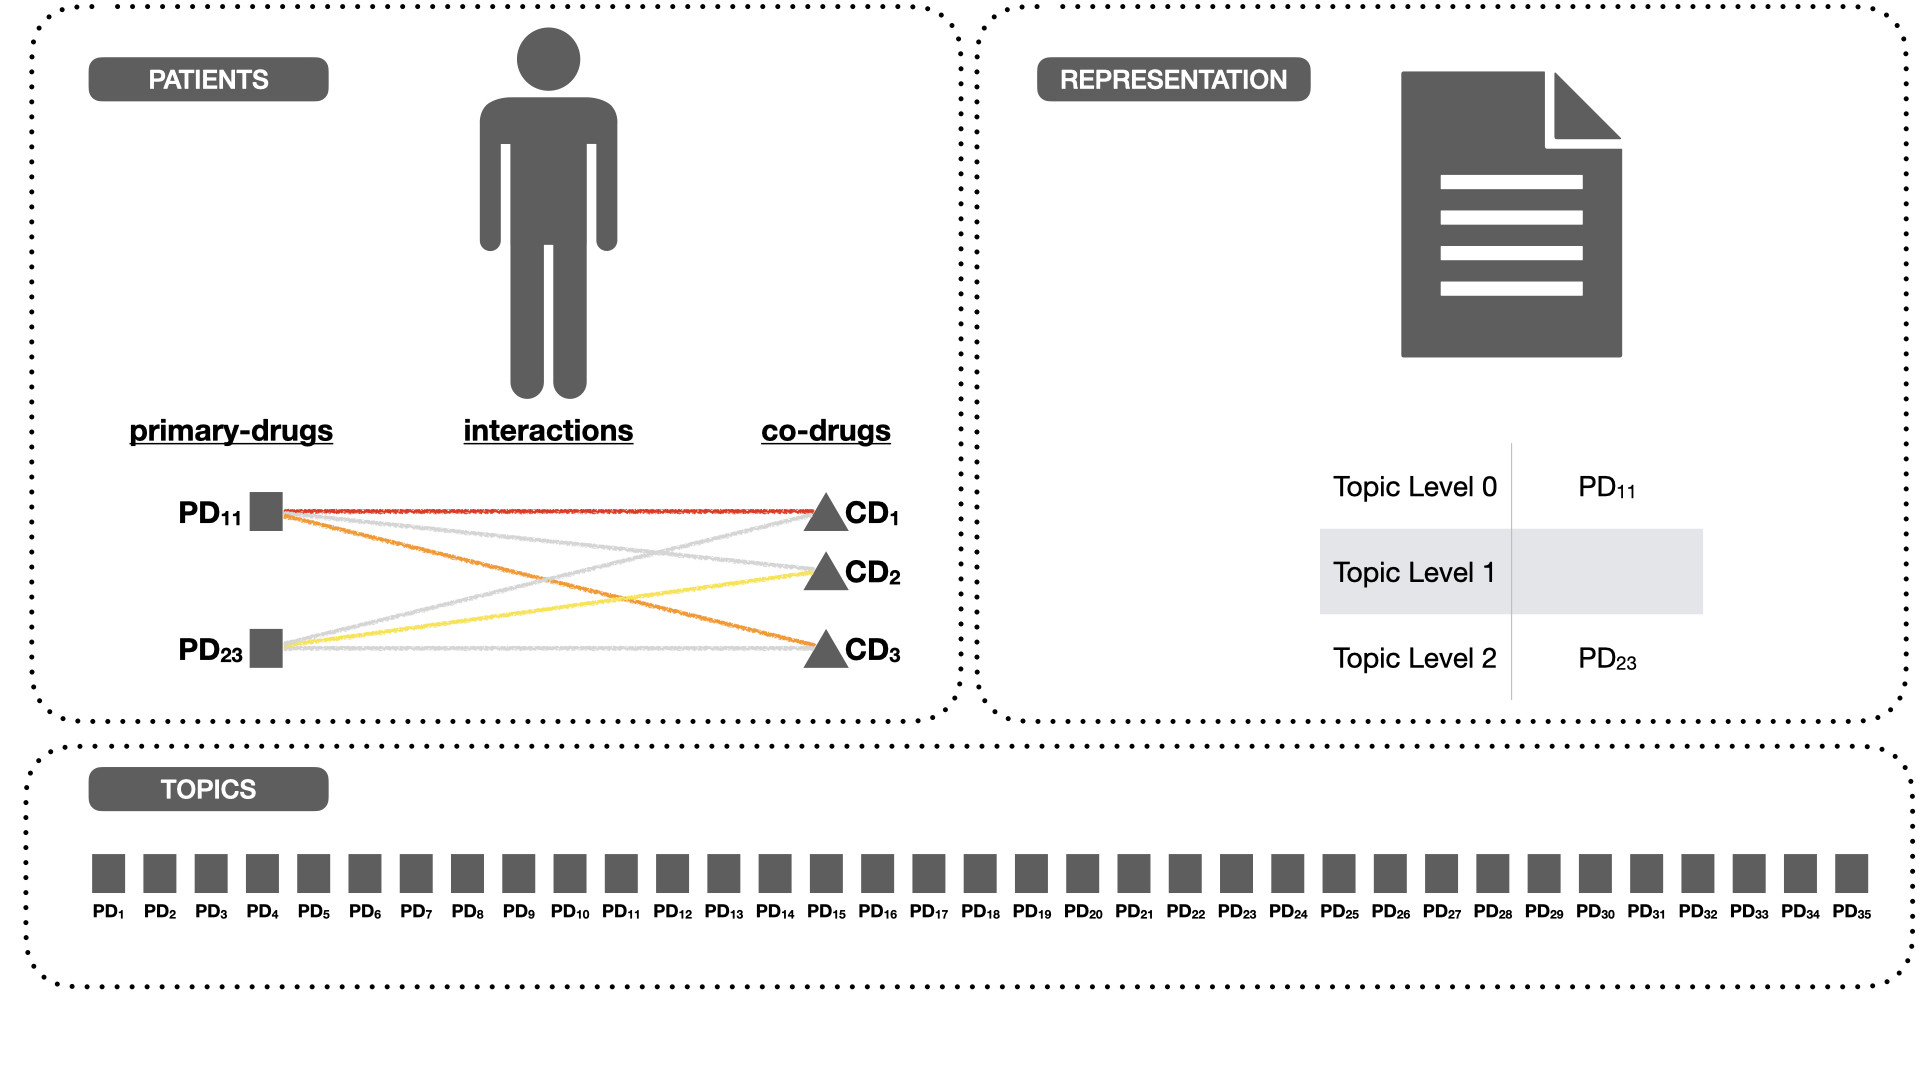
\includegraphics[width=0.8\linewidth]{polypharmacy.png}
    \caption{Representation of patients through topic hierarchies based on the interactions between primary-drugs and co-drugs}
    \label{fig:polypharmacy-topics}
\end{figure}

Specifically, in this work we were able to put into practice our approach to make comparisons (Chapter \ref{ch:comparisons}) when discovering drug–drug interactions (DDIs) in HIV patients. The anonymized registries from the Madrid Health Service (SERMAS) database were used to build a working database with information about all patients who picked up antiretrovirals (ARVs) or non-HIV medications during the study period. A total of 22,945 people living with HIV and 6,613,506 individuals without HIV had received medications. Medications from the SERMAS database were separated into ARVs and non-HIV drugs: 35 primary-drugs (i.e ARVs medications) and 1,058 co-drugs (i.e non-HIV medications). All drug pairs between primary- and co-drugs were interrogated using the University of Liverpool (UoL) Drug Interactions Database\footnote{\url{https://www.hiv-druginteractions.org}}, with more than 24,000 HIV DDIs between ARVs and non-HIV medications, to generate a comprehensive list of potential DDIs. The Liverpool flag classification  categorizes the severity of DDIs as follows: a red flag indicates medications that should not be coadministered as they might lead to serious adverse events or profoundly affect antiretroviral therapy efficacy; an orange flag indicates a potential interaction that might require dosage modification or close monitoring to minimize clinical consequences; a yellow flag indicates a potential interaction of weak relevance not requiring additional monitoring or dosage adjustment; a green flag indicates no anticipated risk of inter-action; and a gray flag indicates no clear data are available to assess whether a DDI will occur.

We built a representation system where each primary-drug was represented as a topic, and each patient was described as a document containing those topics with different weights (Figure \ref{fig:polypharmacy-topics}). This value depends on the DDIs between the primary-drugs and the co-drugs of the patients. Red-flag interactions correspond to the most relevant topics (i.e. level 0), orange-flag interactions correspond to the following topics (i.e. level 1), and yellow-flag interactions correspond to the least relevant topics (i.e. level 2). Primary-drugs are assigned to the most relevant level. Patients are thus described by DDIs, making it easy to identify sets of risks according to the severity of the interactions.


\begin{figure}[ht]\centering
   \begin{minipage}{0.49\textwidth}
     \frame{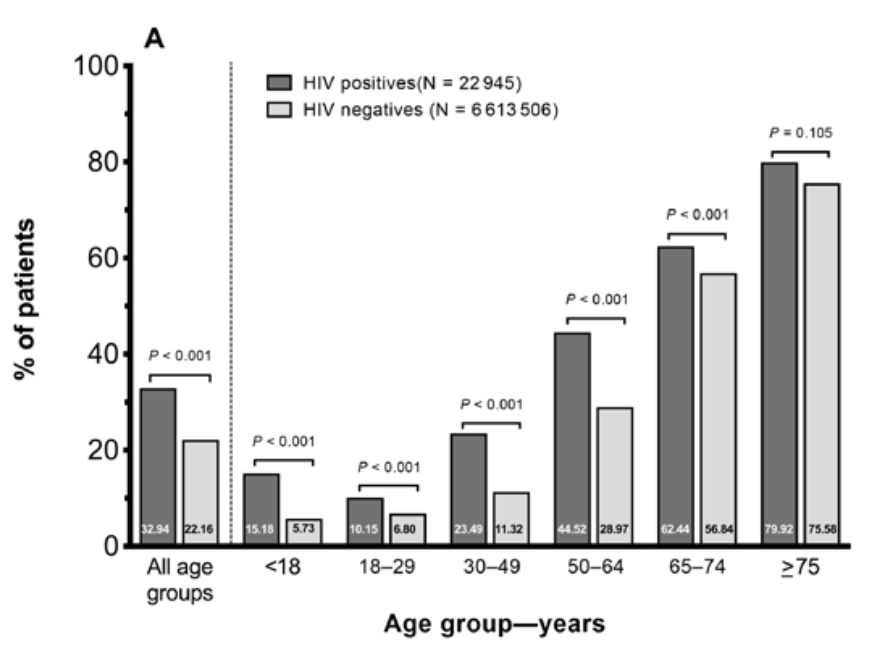
\includegraphics[width=\linewidth]{polypharmacy01.png}}
     \caption{Patients grouped by age}\label{subfig:poly-age}
   \end{minipage}
   \begin {minipage}[c]{0.49\textwidth}
     \frame{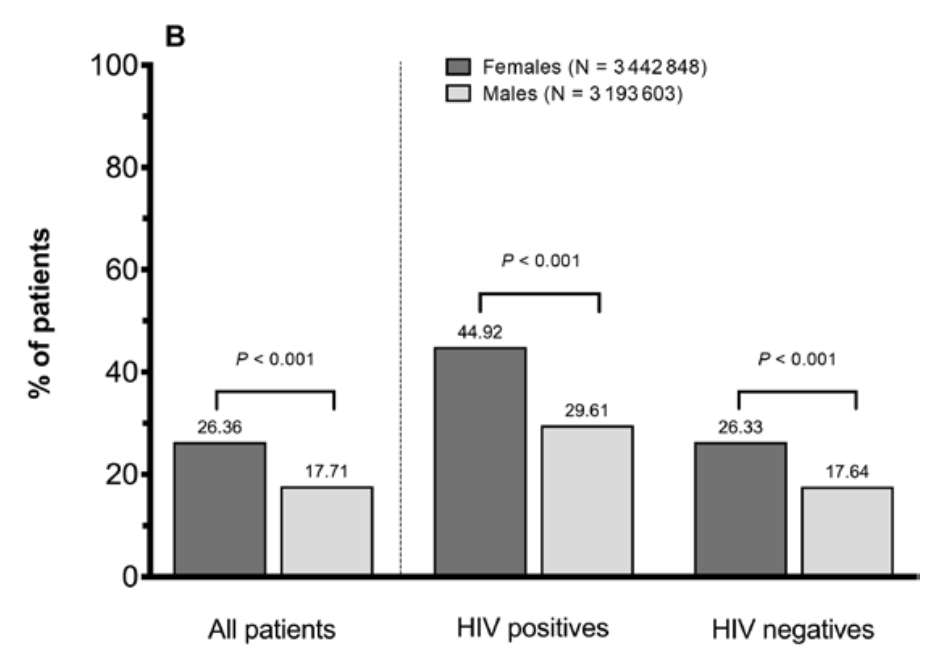
\includegraphics[width=\linewidth]{polypharmacy02.png}}
     \caption{Patients grouped by gender}\label{subfig:poly-gender}
   \end{minipage}
   \caption{Distribution of polypharmacy among people living with and without HIV according to age and gender \citep{Badenes-Olmedo2019c}.}
   \label{fig:polypharmacy}
\end{figure}

Our contribution facilitates the analysis of patients and drugs (interactions) without having to make all the comparisons between them (Figure \ref{fig:polypharmacy}). Patients are grouped by interactions on the same primary medications. The source code we have developed to discover drug interactions is publicly available for reuse\footnote{\url{https://github.com/cbadenes/hiv-ichart-client}}, but for privacy reasons we cannot publish the code to manage patients. 

\section{DrInventor}
\label{sec:drinventor}

Scientific creativity and innovation are key concepts at a time of rapid technological change. Technologies have great potential to supplement human ingenuity in science by overcoming the limitations that people suffer in pursuing scientific discovery. DrInventor\footnote{\url{http://drinventor.eu}} proposes an original system to provide inspiration for scientific creativity by utilizing the rich presence of web-based research resources \citep{Dong2017DrIP}. It is like a personal research assistant that informs researchers of a broad spectrum of relevant research concepts and approaches, by assessing the novelty of research ideas, and by offering suggestions of new concepts and workflows with unexpected features for new scientific discovery.

Our topic modeling framework, librAIry (more details in Chapter \ref{ch:scalability}), and the topic-based characterization to measure the similarity between documents (described in Section \ref{sec:topicmodel}) powered the DrInventor platform to automatically relate scientific publications from their content. We created a harvester module\footnote{\url{https://github.com/cbadenes/camel-oaipmh}} (Section \ref{sec:librairy-modules})  that was able to ingest and index research resources from external sources based on the Open Archive Initiative Protocol for Metadata Harvesting\footnote{\url{https://www.openarchives.org/pmh/}}. The resources were processed at different levels of granularity: from the entire documents, to their individual items, parts or even individual words contained in them. On top of those resources DRInventor attaches different annotations that further described the instances and gave support to different operations leveraging on them. The model (Figure XXX) provided a standard way of representing research documents, and was flexible enough to give support to a great variety of analysis techniques bringing value to the information stored in it. 

\begin{figure}[ht]
    \centering
    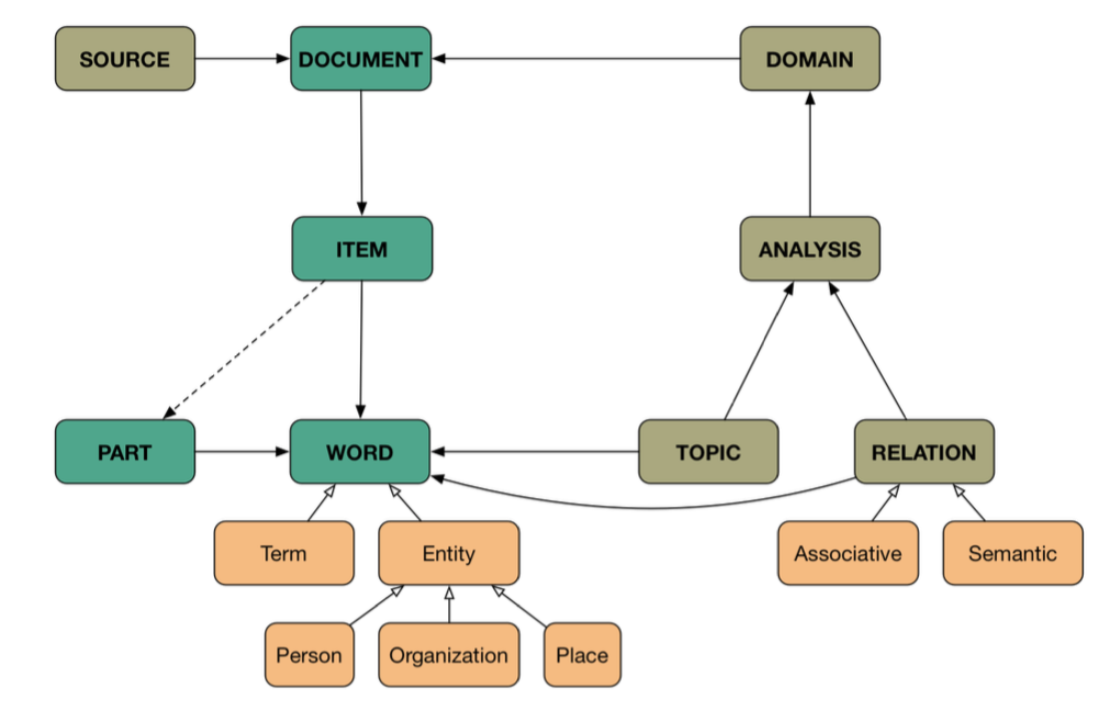
\includegraphics[width=0.8\linewidth]{drinventor-model.png}
    \caption{Overview of Resources in DRInventor Platform}
    \label{fig:drinventor-model}
\end{figure}


The main types of resources (Figure \ref{fig:drinventor-model}) that were considered in DRInventor, from the most fine/grained to the most general ones, were:
\begin{itemize}
\item \textbf{Word}: a meaningful element of writing inside a document, formed by a sequence of characters with no blanks.
\item \textbf{Part}: logical division of a document, based on categories of the research discourse such as abstract, introduction, methods, results, conclusions, etc., including also the types of rhetorical sentences \citep{Ronzano2015} (i.e. approach, background, challenge, future work or outcomes).
\item \textbf{Item}: each of the elements that make up a research object (i.e. a document) such as a paper, programming-code, an image, a workflow, and so on.
\item \textbf{Document}: meta-information retrieved from a research object. A document is composed by a set of \textit{items}.
\item \textbf{Source}: indicates the repository where the raw research objects were collected from a link where the platform can look at in order to retrieve them.
\item \textbf{Domain}: represents the collection of the resources inside DRInventor generated after ingesting the research objects from the repository specified by the \textit{source}.
\item \textbf{Analysis}: it represents the execution of an algorithm over a particular \textit{domain} in the platform. It is responsible for the creation of annotations, such as \textit{topics} and \textit{relations}.
\item \textbf{Term}: represents and abstracts concepts, such as \textit{entities} (persons, locations, organizations...) as results of the execution of different Natural Language Processing algorithms.
\item \textbf{Topic}: helps to materialize the main subjects that the corpus is elaborating on, such as the research areas or trending issues in the scientific domain.
\item \textbf{Relation}: is an associative or semantic connection between resources in a domain. It can model for example the high degree of similarity between two \textit{parts} belonging to different research objects.
\end{itemize}

The DrInventor model served us to refine the model proposed in this thesis (see Section \ref{sec:representing-corpora}). Some resources were eliminated (e.g. \textit{Source}) to minimize the representation elements to those that can be used to create probabilistic topic models and to calculate similarities between documents (e.g. document, domain, annotation). It has also allowed us to generalize our model by adding a \textit{snippet} resource to represent any element (e.g. part, sentence, entity) that may appears in a document.


\section{Corpus Viewer}
\label{sec:corpus-viewer}
...

\section{TheyBuyForYou}
\label{sec:tbfy}
...

\section{Drugs4Covid}
\label{sec:drugs4covid}
...